%! Author = johannes
%! Date = 10/13/21

% Preamble
\documentclass[12pt]{article}
\title{Classical Assignment \#6}
\author{Johannes Byle}

% Packages
\usepackage{amsmath}
\usepackage[margin=0.75in]{geometry}
\usepackage{lipsum}
\usepackage{physics}
\usepackage{ifthen}
\usepackage{tikz}
\usepackage{pgfplots}
\usepackage{graphicx}
\usepackage{csquotes}
\usetikzlibrary{math}
\usetikzlibrary{angles, quotes}

% Commands
\newcommand{\p}[2]{\frac{\partial #1}{\partial #2}}
\newcommand{\der}[2]{\frac{d #1}{d #2}}
\newcommand{\Lag}[3]{
  \p{L}{#1}-\der{}{t}\p{L}{\dot{#1}}=0\\
  \p{L}{#1}=#2,\quad \der{}{t}\p{L}{\dot{#1}}=#3\\
  #2-#3=0
}
\newcommand{\Lagq}[4]{
  \p{L}{#1}-\der{}{t}\p{L}{\dot{#1}}+\lambda\p{f}{r}=0\\
  \p{L}{#1}=#2,\quad \der{}{t}\p{L}{\dot{#1}}=#3,\quad \p{f}{#1}=#4\\
  #2-#3\ifthenelse{#4=1}{+\lambda}{\ifthenelse{#4=0}{+0}{+\lambda#4}}=0
}

% Document
\begin{document}
  \maketitle
  \begin{enumerate}
    \item
    \begin{enumerate}
      \item The effective potential is simply:
      \begin{gather*}
        V_{\text{eff}}(r)=\frac{L^2}{2\mu r^2}-C\frac{e^{-\alpha r}}{r}
      \end{gather*}
      \includegraphics{HW_6_scripts/v_eff}
      \item
      There are 3 distinct ranges of energies:
      The first range of energies are those above the \enquote{hump} where the particle will simply be scattered.
      Below this the particle will either, depending on the initial value of $r$, scatter of the hump, or \enquote{orbit} around the central force while oscillating between two different values of $r$.
      The third range is simply the bottom of the well, the lowest allowed energy, where the particle will cleanly orbit the central force.
    \end{enumerate}
    \item
    \begin{enumerate}
      \item Since the particle is scattering off of a sphere, $r_{\min}=a_0$, and since the origin is at the center of the sphere $\Psi=\arcsin\left( \frac{s}{a_0} \right)$.
      Using the relation $\Theta=\pi-2\Psi$ we get $\Theta=\pi-2\arcsin\left( \frac{s}{a_0} \right)$.
      Rearranging this equation in terms of $s$:
      \begin{gather*}
        s=\sin\left(\frac{\pi-\Theta}{2}\right)=\cos\left( \frac{\Theta}{2} \right)\\
        \der{s}{\Theta}=-\frac{1}{2}\sin\left( \frac{\Theta}{2} \right)
      \end{gather*}
      Plugging this into the equation (3.93) from Goldstein:
      \begin{gather*}
        \sigma(\Theta)=\frac{s}{\sin\Theta}\left| \frac{ds}{d\Theta} \right|=\frac{\cos\left( \frac{\Theta}{2} \right)}{\sin\Theta}\left| \frac{1}{2}\sin\left( \frac{\Theta}{2} \right) \right|=\frac{1}{4}\text{sgn}\left[\sin\left( \frac{\Theta}{2} \right)\right]\\
        \sigma(\Theta)=\frac{1}{4}\quad\text{between 0 and 2}\pi
      \end{gather*}
      Calculating the total cross-section $\sigma_T$:
      \begin{gather*}
        \sigma_T=2\pi\int_0^{\pi} \sigma(\Theta)\sin\Theta d\Theta=\frac{\pi}{2}\int_0^{\pi}\sin\Theta d\Theta=\pi
      \end{gather*}
      This means that the scattering cross-section at every angle would is the same, in the case of an experiment it would mean that the final screen would be completely evenly covered (assuming it's curved around the scattering center).
      \item Since energy is conserved, the particle will move in a different direction when it is inside the sphere, since now part of the energy is taken up by the potential.
      The angle it moves will be governed by the differences in velocity $n=\frac{v_1}{v_0}=\sqrt{1+V_0/E}$.\footnote{http://www.phys.lsu.edu/faculty/gonzalez/Teaching/Phys7221/Hwk6Solns.pdf}\\
      \begin{center}
        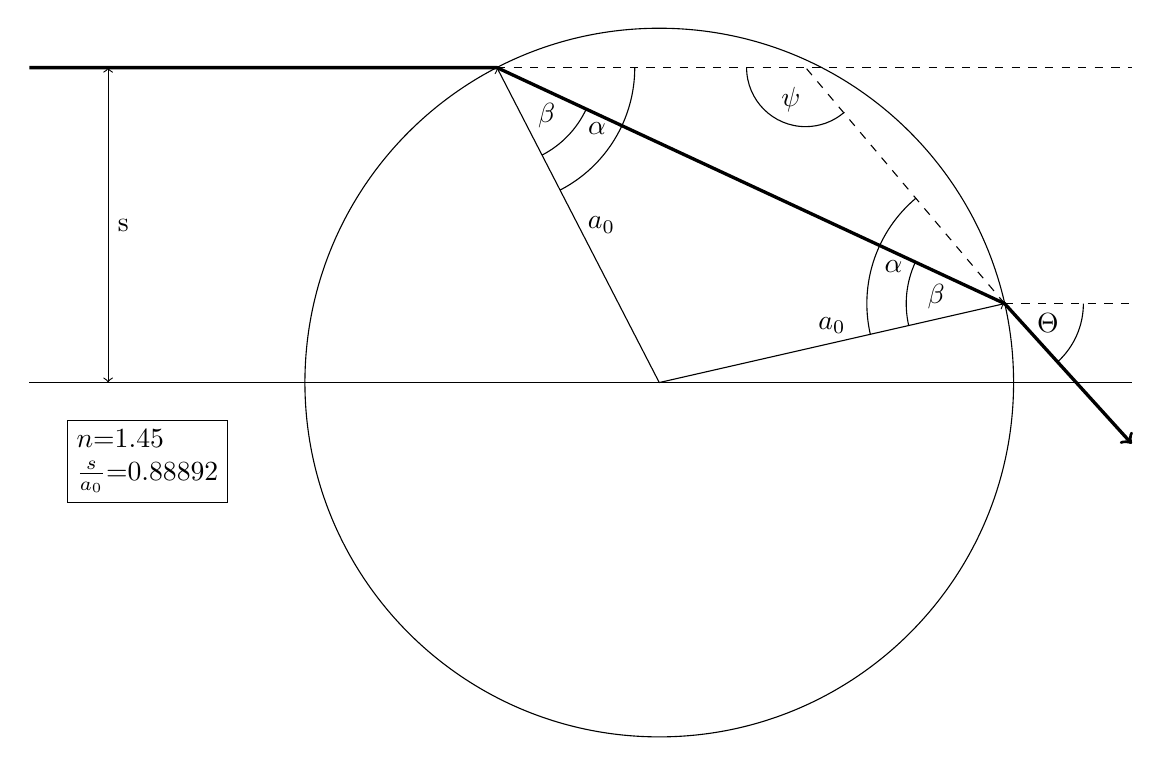
\begin{tikzpicture}
          \tikzmath{
            \n=1.45;
            \s=4;
            \r=4.5;
            \ratio=\s/\r;
            \start=-8;
            \final=6;
            \alph=asin(\s/\r);
            \bet=asin(sin(\alph)/\n);
            \x1=-\r * cos(\alph);
            \d=2*\r*sin((180-(2*\bet))/2);
            \y2=\s-\d*sin(\alph-\bet);
            \x2=\x1+\d *cos(\alph-\bet);
            \thet=2*(\alph-\bet);
            \y3=\y2-((\final-\r) * tan(\thet));}
          \node[draw, align=left] at (\start+1.5,-1) {$n$=\n\\$\frac{s}{a_0}$=\ratio};
          \draw[very thick, ->] (\start,\s) -- (\x1, \s) -- (\x2, \y2) -- (\final, \y3);
          \draw[->] (0,0) --node[anchor=west]{$a_0$} (\x1, \s);
          \draw[->] (0,0) --node[anchor=south]{$a_0$} (\x2, \y2);
          \draw[dashed] (\x1, \s) -- (\final, \s);
          \draw[dashed] (\x2, \y2) -- (\final, \y2);
          \draw[dashed] (\x2,\y2) -- ({\x2-(\s-\y2)*tan(90-\thet)},\s);
          \draw[<->] (\start+1,0) -- node[anchor=west]{s} (-7,\s);
          \draw(-8, 0) -- (\final, 0);
          \draw(0,0) circle (\r);
%                    \coordinate (A) at (\x1,\s);
%                    \coordinate (B) at (0,0);
%                    \coordinate (C) at (\x1,0);
%                    \draw pic [draw,angle radius=0.75cm, "$\alpha$"] {angle};
          \coordinate (A) at (0,0);
          \coordinate (B) at (\x1,\s);
          \coordinate (C) at (\x2,\y2);
          \draw pic [draw,angle radius=1.25cm, angle eccentricity=0.7, "$\beta$"] {angle};
          \coordinate (A) at (\final,\y3);
          \coordinate (B) at (\x2,\y2);
          \coordinate (C) at (\final,\y2);
          \draw pic [draw,angle radius=1cm, "$\Theta$"] {angle};
          \coordinate (A) at (\x1,\s);
          \coordinate (B) at ({\x2-(\s-\y2)*tan(90-\thet)},\s);
          \coordinate (C) at (\final,\y3);
          \draw pic [draw,angle radius=0.75cm, "$\psi$"] {angle};
          \coordinate (A) at ({\x2-(\s-\y2)*tan(90-\thet)},\s);
          \coordinate (B) at (\x2,\y2);
          \coordinate (C) at (0,0);
          \draw pic [draw,angle radius=1.75cm, angle eccentricity=0.85, "$\alpha$"] {angle};
          \coordinate (A) at (0,0);
          \coordinate (B) at (\x1,\s);
          \coordinate (C) at (\x2,\s);
          \draw pic [draw,angle radius=1.75cm, angle eccentricity=0.85, "$\alpha$"] {angle};
          \coordinate (A) at (\x1,\s);
          \coordinate (B) at (\x2,\y2);
          \coordinate (C) at (0,0);
          \draw pic [draw,angle radius=1.25cm, angle eccentricity=0.7, "$\beta$"] {angle};
        \end{tikzpicture}
      \end{center}
      All the angles in this graph be found from the initial parameters $n,\ s,$ and $a_0$:
      \begin{gather*}
        \alpha=\arcsin\left( \frac{s}{a_0}\right),\quad\beta=\arcsin\left( \frac{s}{na_0} \right),\quad\Theta=2(\alpha-\beta)
      \end{gather*}
      The equation for $\Theta$ can be found using the angle $\psi=\pi-2(\alpha-\beta)$ since $\Theta=\pi-\psi$.
      We can solve for $s$ starting with the equation for $\beta$:
      \begin{align*}
        \frac{s}{na_0}&=\sin\beta\\
        s&=na_0\sin\left(\alpha-\frac{\Theta}{2}\right)\\
        s&=na_0\left[\sin\alpha\cos\left(\frac{\Theta}{2}\right)-\cos\alpha\sin\left(\frac{\Theta}{2}\right)\right]\\
        s&=na_0\left[\frac{s}{a_0}\cos\left(\frac{\Theta}{2}\right)-\cos\alpha\sin\left(\frac{\Theta}{2}\right)\right]\\
        s^2&=n^2 a_0^2\left[\frac{s}{a_0}\cos\left(\frac{\Theta}{2}\right)-\cos\alpha\sin\left(\frac{\Theta}{2}\right)\right]^2\\
        s^2&=\frac{a_0^2 n^2\sin^2\left( \frac{\Theta}{2} \right)}{1+n^2-2n\cos\left( \frac{\Theta}{2} \right)}\quad\text{Using }\cos^2\alpha=1-\frac{s}{a_0}\\
        s&=\frac{a_0 n\sin\left( \frac{\Theta}{2} \right)}{\sqrt{1+n^2-2n\cos\left( \frac{\Theta}{2} \right)}}
      \end{align*}
    \end{enumerate}
    \item
    \begin{enumerate}
      \item Starting with the equation for $\Theta$, using $du=-\frac{1}{r^2}dr$ and $V(r)=-\frac{k}{2r^2}$:
      \begin{align*}
        \Theta(s,E)&=\pi-2\int_0^{u_{\max}}\frac{sdu}{\sqrt{1-\frac{V(u)}{E}-s^2 u^2}}\\
        \Theta(s,E)&=\pi-2\int_{r_{\min}}^{\infty}\frac{-s\frac{1}{r^2}}{\sqrt{1-\frac{V(\frac{1}{r})}{E}-s^2\frac{1}{r^2}}}dr\quad\text{Replacing $u$ terms}\\
        \Theta(s,E)&=\pi-2\int_{r_{\min}}^{\infty}\frac{-\frac{s}{r^2}}{\sqrt{1+\frac{kr^2}{2E}-\frac{s^2}{r^2}}}dr\quad\text{Substituting $V(r)$}\\
        \Theta(s,E)&=\pi-2\int_{r_{\min}}^{\infty}\frac{sdr}{r\sqrt{r^2\left(1+\frac{k}{2r^2 E}\right)-s^2}}
      \end{align*}
      $r_{\min}$ is determined by the angular momentum, thus $E=\frac{L^2}{2\mu r_{\min}}$ and $r_{\min}=\sqrt{\frac{L^2}{2\mu E}}$:
      \begin{align*}
        \Theta(s,E)&=\pi-2\int_{r_{\min}}^{\infty}\frac{sdr}{r\sqrt{r^2\left(1+\frac{k}{2r^2 E}\right)-s^2}}\\
        \Theta(s,E)&=\pi-2\int_{\sqrt{\frac{L^2}{2\mu E}}}^{\infty}\frac{sdr}{r\sqrt{r^2\left(1+\frac{k}{2r^2 E}\right)-s^2}}\\
        \Theta(s,E)&=\pi\left[1-\frac{s\sqrt{2E}}{\sqrt{k+2Es^2}}\right]
      \end{align*}
      \item
      \begin{align*}
        \der{^2u}{\theta^2}+u&=-\frac{m}{l^2}\der{}{u}\left(-\frac{ku^2}{2}\right)\\
        \der{^2u}{\theta^2}+u&=-\frac{m}{l^2}ku\\
        \der{^2u}{\theta^2}&=u\left(\frac{mk}{l^2}+1\right)\\
      \end{align*}
      This is a common differential equation:
      \begin{gather*}
        u(\theta)=\alpha\cos\left(\sqrt{1+\frac{mk}{l^2}}\theta  \right)+\beta\sin\left(\sqrt{1+\frac{mk}{l^2}}\theta  \right)\\
        u(\theta)=\alpha\cos\left(\gamma\theta  \right)+\beta\sin\left(\gamma\theta  \right)\\
      \end{gather*}
      \item
      \begin{enumerate}
        \item Using the fact that $u'(\theta)=\beta\gamma\cos(\gamma\theta)-\alpha\gamma\sin(\gamma\theta)$:
        \begin{gather*}
          u(\pi)=\alpha\cos(\gamma\pi)+\beta\sin(\gamma\pi)=0\\
          u'(\pi)=\beta\gamma\cos(\gamma\pi)-\alpha\gamma\sin(\gamma\pi)=0
        \end{gather*}
        The first expression is simple to show from the first equation:
        \begin{align*}
          \alpha\cos(\gamma\pi)&=-\beta\sin(\gamma\pi)\\
          \alpha=-\beta\tan(\gamma\pi)
        \end{align*}
        \item The second expression takes some work:
        \begin{align*}
          \beta\gamma\cos(\gamma\pi)&=\alpha\gamma\sin(\gamma\pi)\\
          \frac{\beta}{\alpha}&=\tan(\gamma\pi)\\
          \frac{\beta}{-\beta\tan(\gamma\pi)}&=\tan(\gamma\pi)\quad\text{Using the expression we found earlier}\\
          \frac{\atan(1)}{\pi}&=\gamma\\
          \frac{1}{4}&=\gamma
        \end{align*}
      \end{enumerate}
      \item Starting with $x=\frac{\Theta}{\pi}$ and the definition of $\Theta$:
      \begin{align*}
        \Theta(s,E)&=\pi\left[1-\frac{s\sqrt{2E}}{\sqrt{k+2Es^2}}\right]\\
        \frac{\Theta(s,E)}{\pi}&=\left[1-\frac{s\sqrt{2E}}{\sqrt{k+2Es^2}}\right]=x\\
        s^2&=\frac{k(1-x)^2}{2E(x-2)x}
      \end{align*}
      Taking a total derivative of both sides:
      \begin{align*}
        2sds&=-\frac{k(x-1)}{E(2-x)^2 x^2}dx\\
        sds&=-\frac{k(x-1)}{2E(2-x)^2 x^2}dx
      \end{align*}
      Plugging this into equation (3.93):
      \begin{gather*}
        \sigma(\Theta)=\frac{s}{\sin\Theta}\left| \frac{ds}{d\Theta} \right|\\
        \sigma(\Theta)d\Theta=\frac{k(x-1)dx}{E(2-x)^2 x^2\sin\Theta}=\frac{k}{E}\frac{(x-1)dx}{(2-x)^2 x^2\sin(\pi x)}\\
      \end{gather*}
    \end{enumerate}
    \item This paper compared Rutherford and hard sphere scattering to the scattering of a hard paraboloid.
    The paper compares the scattering cross sections of a paraboloid and a sphere to show that for different values of $\theta$ the paraboloid cross section either is zero or resembles the Rutherford cross section.
    The paper then discusses how to find paraboloid equivalent to Rutherford scattering for a given energy by deriving the formula $d=k/2T_0(1-\cos\theta)$, where $k/2T_0$ is the parameter governing the shape of the parabola.
    The paper also visually compares the hard sphere to the paraboloid to show visually whey they are similar for certain angles.
  \end{enumerate}


\end{document}